\chapter{Results} \label{ch:results}
For this section, the general training structure will be discussed. This training scheme serves the purpose of training the agent, such that its value function will converge at an optimal policy. The agent was faced with a random walk policy at each game. But to even the odds then the random walk policy was never allowed to buy curses which significantly boosted its win chance. 



\section{Training amounts}
Training a dominion gamed until convergence usually lasted around 48 hours. This meant that training was doable, but not replicable, as it would take too long. Convergence happened at around 2000 games. To get reliable data, then instead of training a single agent op to 2000 games, the agent is trained in 20 epochs with 150 games. The return gained from each game will then be averaged to reduce variance in the results of the methods.
\section{Results}
The section is dedicated to the results of this project. Figure \ref{fig:winrate_graph} shows the average winrate graph of all agents. The agent has trained in 150 games, and 15 epochs. The performance is evaluated after every 4 training games. The amount of performance games is therefore $150/4 = 37$ games.

In the Github repository for this project, then all the game logs can be found \footnote{https://github.com/Pengu20/Dominion\_AI/tree/main/game\_history}. These game logs are also used in the discussion and evaluation of the game.
Figure \ref{fig:discounted_returns} shows the discounted returns of all three agents.

The average winrate for all three agents are as follows:
\begin{itemize}
    \item SARSA: 69.82 \%
    \item Q-learning: 65.96 \%
    \item Expected SARSA: 74.91 \%
\end{itemize}

\begin{figure}[H]
    \centering
    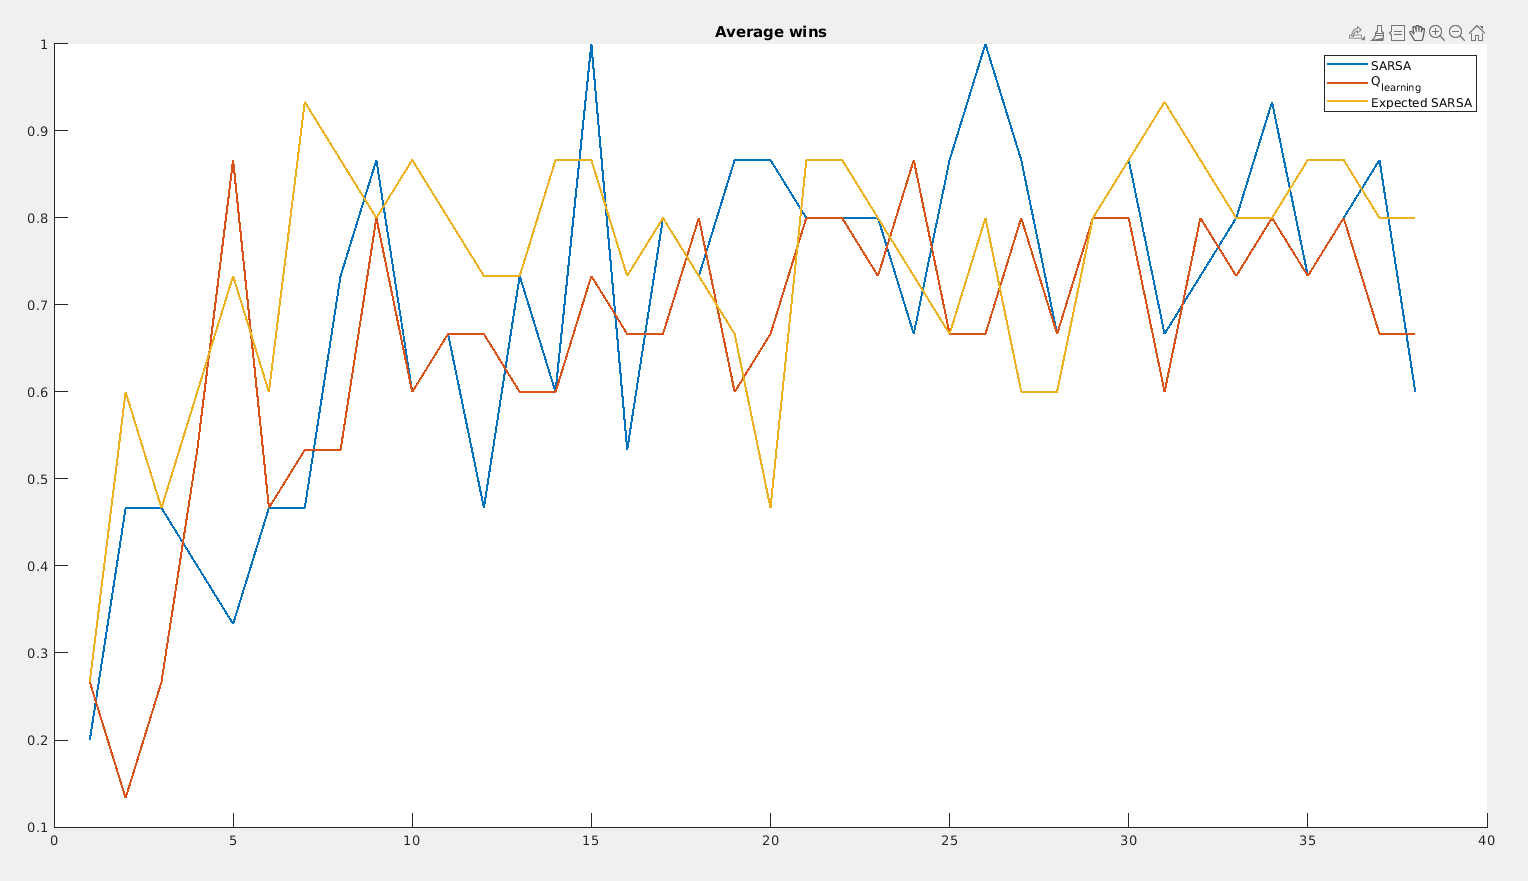
\includegraphics[width=\linewidth]{img/Win_rate_graph.png}
    \caption{This figure shows the winrate of all three methods based on 20 epochs with 150 games each. The x-axis is performance game, and y axis is winrate}
    \label{fig:winrate_graph}
\end{figure}


\begin{figure}[H]
    \centering
    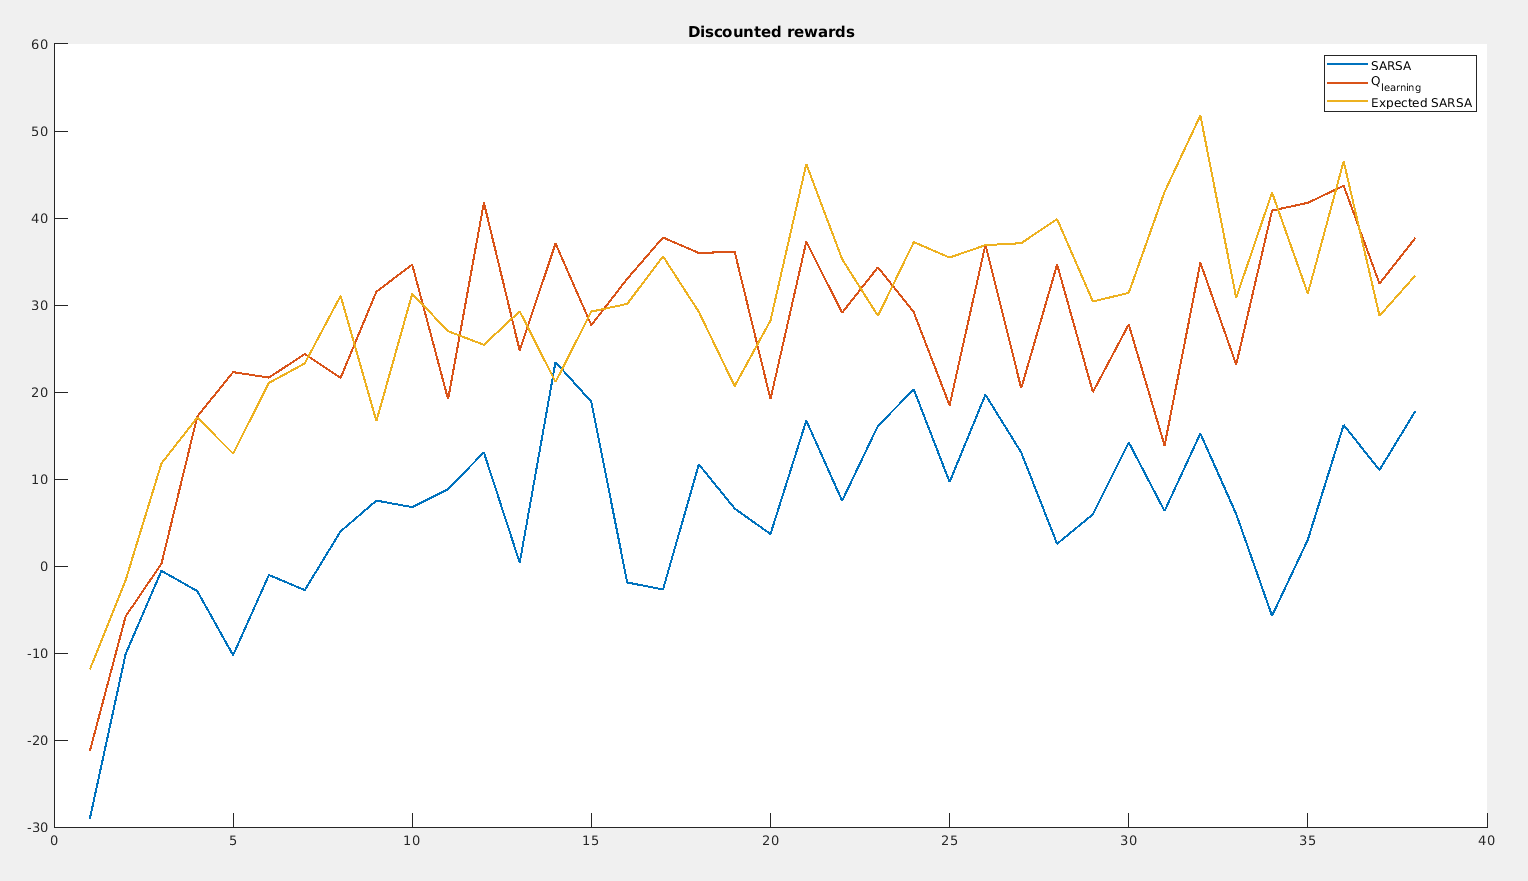
\includegraphics[width=\linewidth]{img/Discounted_rewards.png}
    \caption{This figure shows the discounted returns for all three methods based on 20 epochs with 150 games each. The x-axis is performance ga}
    \label{fig:discounted_returns}
\end{figure}
